\subsubsection{Divide-and-Conquer-Verfahren}
\label{ssub:voronoiAlgorithmsDivAndConq}
Gemäss~\citeauthor{goodrich2002algorithm} besteht das Divide-and-Conquer-Verfahren (zu Deutsch ``Teile und Herrsche'') grundsätzlich aus drei Schritten:

\begin{compactitem}
\item \textbf{Divide (Teilen)}: Ist ein (Teil-) Problem kleiner als ein gewisser Schwellwert (z.B. ein oder zwei Elemente), wird das (Teil-) Problem mit einer direkten Methode gelöst und danach das Resultat zurückgegeben. Andernfalls wird das (Teil-) Problem in zwei oder mehrere, möglichst gleichgrosse Teilprobleme aufgeteilt (\citeyear{goodrich2002algorithm}, S. 210).

    \item \textbf{Recur (Wiederholen)}: Die Teilprobleme werden rekursiv gelöst.

    \item \textbf{Conquer (Erobern)}: Die Lösungen der Teilprobleme werden zu einer Gesamtlösung des ursprünglichen Problems zusammengefügt (ebd.).

\end{compactitem}

Nach~\citeauthor{shamos1975closestpoint} kann das Divide-and-Conquer-Verfahren zur Erzeugung eines Voronoi-Diagramms $V(S)$ eingesetzt werden. Ein zentraler Aspekt ist hierbei, die $n$-elementige Menge $S$ mittels sogenannten \textit{\textbf{Splitgeraden}}, welche horizontal oder vertikal sind, in Teilmengen zu zerteilen (S. 151 bis 162).

Laut~\citeauthor{klein2005algorithmischegeometrie} führt dies zu folgendem Initialisierungsaufwand für den \textbf{Divide-Schritt}: ``Nach $O(n \log{n})$ Vorbereitungszeit lässt sich die Punktemenge $S$ rekursiv durch achsenparallele Splitgeraden so zerlegen, dass jeder Zerlegungsschritt einer Teilmenge $T$ in Zeit $O(|T|)$ ausgeführt werden kann und zwei Teilmengen mit Mindestgrösse $1/4(|T| - 1)$ liefert'' (\citeyear{klein2005algorithmischegeometrie}, S. 295).

Ein weiterer zentraler Aspekt ist nun die Frage, wie schnell sich zwei Voronoi-Diagramme, z.B. $V(R)$ und $V(S)$ zu einem gemeinsamen Voronoi-Diagramm, also $V(R \in S)$, zusammensetzen (\textbf{Conquer-Schritt}) lassen. Hierzu müssen zwei Arten von Voronoi-Kanten unterschieden werden: Kanten, deren Punkte zu derselben Teilmenge $R$ oder $S$ gehören und Kanten, die zwischen den beiden Regionen verlaufen. Diese Kanten bilden den Bisektor der beiden Teilmengen $B(R,S)$, oder, laut dem Autor~\citeauthor{klein2005algorithmischegeometrie}: ``$V(R)$ und $V(S)$ werden mit dem Faden $B(R,S)$ zusammengenäht, und die überstehenden Stücke werden abgeschnitten''. Die schwierigste Aufgabe ist also die Konstruktion des Bisektors. Alle anderen Schritte können dann in der Zeit $O(n)$ vorgenommen werden~\parencite[S. 297 bis 298]{klein2005algorithmischegeometrie}.

\newpage{}

\begin{figure}[h]
\centering
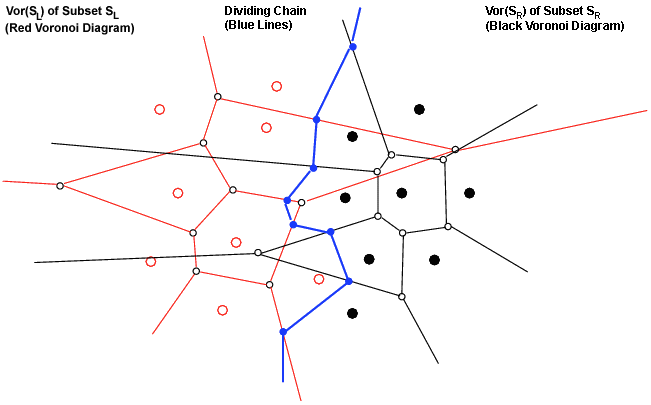
\includegraphics[width=200px]{images/voronoi_divide_conquer_01.png}
\caption{Beispiel des Bisektors $B(R,S)$\protect\footnotemark, blau dargestellt}
\label{fig:voronoiRegionExample01}
\end{figure}
\footnotetext{\cite{rmuhamma2010}}

Das Erstellen des Bisektors der beiden Voronoi-Regionen geschieht in zwei Phasen. Zuerst wird eines der unbeschränkten Endstücke von $B(R,S)$ gesucht, dann verfolgt man den Bisektor durch beide Voronoi-Diagramme $V(R)$ und $V(S)$ bis man bei dem anderen Endstück von $B(R,S)$ angelangt ist.

Um eines der unbeschränkten Endstücke von $B(R,S)$ zu finden, werden die beiden Regionen $V(R)$ und $V(S)$ quasi übereinandergelegt. Dabei kann der Durchschnitt zweier unbeschränkter Regionen $VR(p, R) \cap VR(q, S)$ leer, beschränkt oder aber unbeschränkt sein. Die unbeschränkten Durchschnitte werden der Reihe nach besucht und es wird getestet ob ein unbeschränktes Stück von $B(R,S)$ darin vorkommt. Ist dies der Fall, so wurde ein Endstück von $B(R,S)$ gefunden. Daraus folgt, wie \citeauthor{klein2005algorithmischegeometrie} sagt: ``Sind $V(L)$ (hier $V(R)$) und $V(R)$ (hier $V(S)$) vorhanden, so lässt sich ein Endstück von $B(L,R)$ (hier $B(R,S)$) in Zeit $O(n)$ finden''~\parencite[S. 298 bis 299]{klein2005algorithmischegeometrie}.

Bei der zweiten Phase geht es nun um die Weiterverfolgung des Bisektors $B(R,S)$ durch die beiden Diagramme $V(R)$ und $V(S)$. Grundsätzlich wird nun eine konvexe Hülle der beiden Diagramme erzeugt, danach wird folgendes Schema angewendet bis der Bisektor, bzw.\ das andere unbeschränkte Endstück, erreicht ist:

\begin{compactitem}
  \item Bisektor $B(r,s)$ der gerade betrachteten Punkte finden
  \item Für den Bisektor wird nun Folgendes bestimmt:
  \begin{compactitem}
    \item der Schnittpunkt $r$ mit der Region $V(R)$, an welchem der Bisektor im letzten Schritt nicht abgeschnitten wurde
    \item der Schnittpunkt $s$ mit der Region $V(S)$, an welchem der Bisektor im letzten Schritt nicht abgeschnitten wurde
    \item die Nachbaren $r'$ und $s'$, welche mit den Schnittpunkten $R$ und $S$ des Bivekorts die Kante gemeinsam haben, auf welcher $r$ und $s$ liegen
  \end{compactitem}
\end{compactitem}

Ist nun der Schnittpunkt $s$ höher als $r$, wird $V(S)$ durch $s'$ ersetzt und der aktuelle betrachtete Bisektor $B(r,s)$ an dem Schnittpunkt $s$ abgeschnitten.
Ist aber der Schnittpunkt $r$ höher als $s$, wird $V(R)$ durch $r'$ ersetzt und der aktuelle betrachtete Bisektor $B(r,s)$ an dem Schnittpunkt $r$ abgeschnitten.
Danach wird der neue aktuelle Bisektor $B(r,s)$ gemäss obigem Schema bestimmt.

Es ist möglich, dass der Bisektor eine Region mehrfach besucht und dabei dasselbe Stück des Randes mehrfach durchläuft, was zu einer höheren Komplexität führt. Es genügt jedoch die linken unbeschränkten Regionen \textit{im Uhrzeigersinn} und die rechten unbeschränkten Regionen \textit{gegen den Uhrzeigersinn} zu durchlaufen und sich dabei den zuletzt gefundenen und verworfenen Schnittpunkt als Abbruchbedingung zu merken (Details siehe~\cite[S. 301]{klein2005algorithmischegeometrie}).

Somit lässt sich ein Voronoi-Diagramm aus $n$-Punkten in einer Ebene in der Zeit $O(n \log{n})$ und linearem Speicherplatz konstruieren~\parencite[S. 299 bis 302]{klein2005algorithmischegeometrie}.
